\section{Network Configuration} \label{sec:Network Configuration}

We introduce our system. We define a temporalliquid state machine (TLSM) as an
input vector, encoded in time-based spikes, followed by a reservoir of temporal
neurons, and finally a singular output column (with winner-takes-all lateral
inhibition). The input vector uses encoding strategies discussed in
\cite{Encoding}, and the output column is identical to the one described in
\cite{TNN}.

\begin{figure}[h]
    \centering
    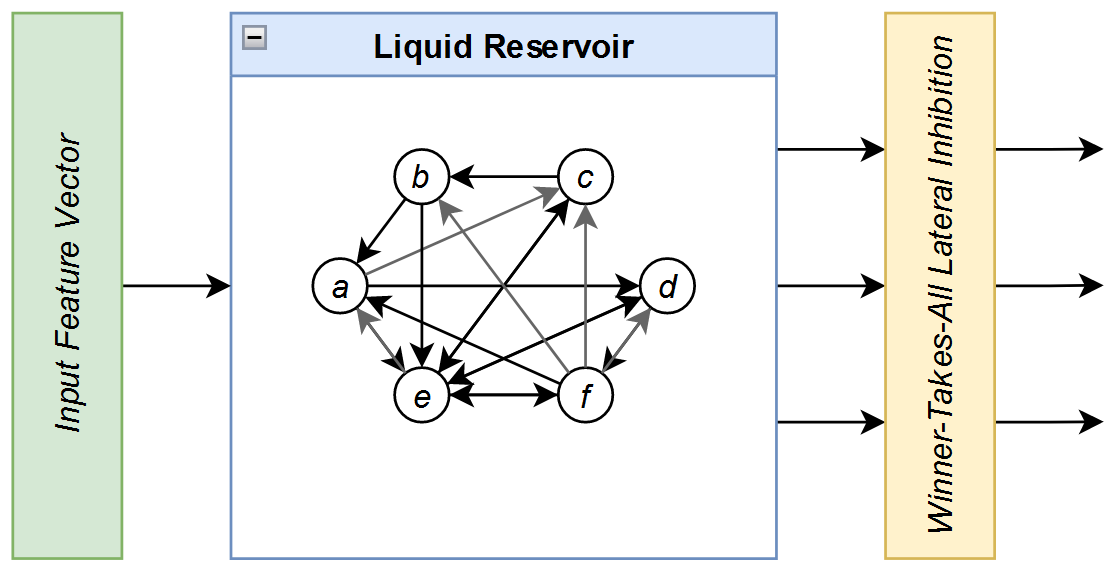
\includegraphics[scale=0.25]{tlsm_diagram.png}
    \caption{Diagram of a temporal liquid state machine (TLSM).}
    \label{fig:tlsm_diagram}
\end{figure}

\subsection{Input Encoding}

The input vector is a series of time-encoded one-hot vector spikes. For the
example of MNIST data, the input $28 \times 28$ image is flattened into a
$784 \times 1$ vector. Each element of the vector is subsequently expanded into
a $t_{res} \times 1$ one-hot time-spike encoding vector, where the time
represents the pixel's brightness. If the pixel is simply black, the time is
set to infinity; Any low values will round to zero. More input processing may
be necessary for particular problems - In order to ensure that bright pixels do
not 'dominate' the input, the image may be duplicated and inverted to include a
pos-neg encoding scheme.

The temporal resolution, $t_{res}$, is an important hyperparameter of this
encoding scheme, as with higher resolutions the network may take longer to train
and infer. However, as resolution increases, so too does accuracy.

\subsection{Temporal Neuron}

The temporal neuron is a simple model of a neuron that fires in response to a
series of time-spiking encoded inputs. It is mainly discussed in \cite{TNN}, but
we will briefly summarize its functionality here. Chiefly, the temporal neuron
consumes significantly less power than point-integrator alternatives, and is
generally trained in an unsupervised fashion. The temporal neuron is also
considered a more biologically plausible neuron model, as it more closely
relates to the Hodgkin-Huxley model \cite{Hodgkin-Huxley} of a neuron.

The temporal neuron takes in a series of inputs on a number of lines, generally
encoded in a one-hot manner. Each line has an internal weight represented with
it, encoding the dendritic segment's channel strength from the pre-synaptic
neuron. The input lines are multiplied and summed, and the result increases the
neuron's body potential. When the body potential reaches a threshold $\theta$,
the neuron will spike, sending a high signal on its axonal output line, and the
body potential will reset.

The method in which neurons accumulate body potential is a hyperparameter of the
network. The simplest implementation strategy is Step No-Leak (SNL) neurons,
where the body potential instantly adds. A more involved strategy is the
Ramp No-Leak (RNL) neuron, where the body potential will increase over time
corresponding to the input. The Leaky Integrate-and-Fire (LIF) neuron is a more
biologically plausible model as well, where the body potential will (in addition
to the ramping nature of the RNL neuron) 'leak' out over time, decreasing the
excitation rate.

\subsection{STDP Training}

We implement Spike-Timing-Dependent Plasticity (STDP) training rules for the
temporal neurons within our work. STDP rules are based closely on Hebbian theory
\cite{STDP}, though the actual definitions of the rules vary. For our
implementation, we utilize unsupervised STDP rules as well as supervised STDP
rules as proposed in \cite{TNN} for some input spike time $t_i$ and output time
$t_j$:

$$
    \Delta w_{ij} = \begin{cases}
        \begin{matrix}
            B(\mu_c)  & \text{ if } t_i\leq t_j, & t_i\neq \infty, & t_j\neq\infty \\
            -B(\mu_b) & \text{ if } t_i > t_j,   &                 & t_j\neq\infty \\
            B(\mu_s)  & \text{ if }              & t_i\neq \infty, & t_j=\infty
        \end{matrix}
    \end{cases}
$$

The parameters of $\mu_c$, $\mu_b$, and $\mu_s$ are the STDP capture, backoff,
and search parameters. They represent finite probabilities, and the notation of
$B(\mu_*)$ refers to the choosing of a Bernoulli random variable. This
implementation of STDP is unsupervised; \cite{TNN} also proposes a supervised
approach to training called R-STDP, which will be used for an output layer.

\subsection{Reservoir}

The reservoir is the focus of network analysis, containing a series of temporal
neurons arranged in a randomly connected graph, or a 'liquid'. This graph of
neurons will change over time with training and with STDP rules, adding and
removing connections arbitrarily in response to the inputs.

Furthermore, a 'seed' configuration for the network may be specified, indicating
its initial connectivity. This seed configuration $W_0$ is generated through a
number of random graph algorithms, and is a hyperparameter of the network.

\subsection{Discriminant Column}

The output discriminating column, responsible for classifying the state of the
liquid, is implemented as a TNN minicolumn as described in \cite{TNN}. The
minicolumn is a series of $n$ neurons (for $n$ output classifications), and is
furthermore fed into a winner-takes-all lateral inhibition (WTA-LI) layer. The
WTA-LI layer implements the biological function of astroglia, inhibiting outputs
of neurons as necessary. STDP rules for this output column also take into
account the output time $t_j$ as the time when the entire column spikes.

With the WTA-LI column, the first neuron to spike inhibits all other neurons,
and will dominate the output. Other forms of inhibition and astrocyte modelling
have been explored in related work (see \cite{Astrocyte}), but will not be
explored within our project.